
%%%%%%%%%%%%%%%%
%%%%%%%%%%%%%%%%

\section{An improved DEC analysis} \label{sec:bg_epoch}

In this section, we'll introduce a suite of model features that lend towards more realistic biogeographic analyses.
Topics include applying range size constraints, stratified (or epoch) models of paleoconnectivity, function-valued dispersal rates, and incorporating uncertainty in paleogeographic event time estimates.
These modifications should produce more realistic ancestral range estimates, e.g. that a volcanic island may only be colonized once it has formed, and that distance should have some bearing on dispersal rate.

To accomplish this, we'll incorporate (paleo-)geographical data for the Hawaiian archipelago, summarized in Table \ref{tab:paleogeo}.
Even though we will continue to use four areas (K, O, M, H) in this section, we will use all six areas (R, K, O, M, H, Z) in Section \ref{sec:bg_phylo}, hence the full table is given for future reference.

\begin{table}[!h]
\centering
\begin{tabular}{l|c|cc|cccccc}
area & code & $a_{max}$ & $a_{min}$ & $g_{\bullet R}$ & $g_{\bullet K}$ & $g_{\bullet O}$ & $g_{\bullet M}$ & $g_{\bullet H}$  & $g_{\bullet Z}$ \\ \hline
Older islands & R & - & - & - & 261 & 406 & 500 & 680 & 3900 \\
Kauai & K & 5.15 & 5.05 & - & - & 145 & 239 & 419 & 3900 \\
Oahu & O & 3.7  & 2.2  & - & -  & -  & 059 & 239 & 3900 \\
Maui Nui & M & 1.8  & 1.3  & - & -  & -  & -  & 082 & 3900 \\
Hawaii & H & 0.7  & 0.3  & - & -  & -  & -  & - & 3900 \\
Mainland & Z & - & - & - & - & - & - & - & - \\
\end{tabular}
\caption{Hawaiian paleogeographic data.
The six areas are given in Figure \ref{fig:hawaii_areas}.
Ages $a_{max}$ and $a_{min}$ report the maximum and minimum origination times for the given island.
Distances $g_{ij}$ report the shortest geographical distance from the coast of the row's area to the column's area (measured at present).}
\label{tab:paleogeo}
\end{table}

\subsection*{Analysis}

Start by creating variables for the tree file, the range data, and the output prefix

\begin{snugshade}
\begin{lstlisting}
range_fn = "data/n4/silversword.n4.range.nex"
tree_fn = "data/n4/silversword.tre"
out_fn = "output/epoch"
\end{lstlisting}
\end{snugshade}

The paleogeographical information from Table \ref{tab:paleogeo} is encoded in three files named {\tt hawaii.n4.times.txt}, {\tt hawaii.n4.distances.txt}, and {\tt hawaii.n4.connectivity.*.txt}.

\begin{snugshade}
\begin{lstlisting}
geo_fn = "data/n4/hawaii.n4"
times_fn = geo_fn + ".times.txt"
dist_fn = geo_fn + ".distances.txt"
\end{lstlisting}
\end{snugshade}

Create move index ({\tt mvi}) and monitor index ({\tt mni}) variables to populate the elements of our {\tt moves} and {\tt monitors} vectors, respectively.

\begin{snugshade}
\begin{lstlisting}
mvi = 1
mni = 1
\end{lstlisting}
\end{snugshade}


Read in the presence-absence range characters and record the number of areas in the dataset

\begin{snugshade}
\begin{lstlisting}
dat_range_01 = readDiscreteCharacterData(range_fn)
n_areas <- dat_range_01.nchar()
\end{lstlisting}
\end{snugshade}

Often, biogeographers wish to limit to the maximum allowable range size.
This prohibits widespread species ranges and reduces the total number of range states in the analysis, thus improving computational efficiency.
We will restrict ranges from including more than two areas.
The total number of ranges equals $\sum_{k=0}^m {{n}\choose{k}}$ where $n$ is the total number of areas, $m$ is the maximum number of permissible areas, and ${{n}\choose{k}}$ is the number of ways to sample $k$ unordered areas from a pool of $n$ areas.
For $n=4$ and $m=2$, this equals ${{4}\choose{0}} + {{4}\choose{1}} + {{4}\choose{2}} = 1 + 4 + 6 = 11$ states.

\begin{snugshade}
\begin{lstlisting}
max_areas <- 2
n_states <- 0
for (k in 0:max_areas) n_states += choose(n_areas, k)
\end{lstlisting}
\end{snugshade}

Then format the dataset for the reduced state space, as provided by {\tt n\_states}

\begin{snugshade}
\begin{lstlisting}
dat_range_n = formatDiscreteCharacterData(dat_range_01, "DEC", n_states)
\end{lstlisting}
\end{snugshade}

Our state space now includes only 11 states ($\emptyset$, K, O, M, H, KO, KM, OM, KH, OH, MH).

As with the previous analysis, we'll assume we know the dated species phylogeny without error.

\begin{snugshade}
\begin{lstlisting}
tree <- readTrees(tree_fn)[1]
\end{lstlisting}
\end{snugshade}

% read in some geography data
Next, we'll read and structure our paleogeographic data.
Read in the list of minimum and maximum ages of island formation

\begin{snugshade}
\begin{lstlisting}
time_bounds <- readDataDelimitedFile(file=times_fn, delimiter=" ")
n_epochs <- time_bounds.size()
\end{lstlisting}
\end{snugshade}

Read in the vector of matrices that describe the connectivity between areas over time.
Note, there is one connectivity matrix per epoch, ordered from oldest to youngest.

\begin{snugshade}
\begin{lstlisting}
for (i in 1:n_epochs) {
  epoch_fn[i] = geo_fn + ".connectivity." + i + ".txt"
  connectivity[i] <- readDataDelimitedFile(file=epoch_fn[i], delimiter=" ")
}
\end{lstlisting}
\end{snugshade}

Read in the matrix of distances between all pairs of areas (km).
For simplicity, we will assume that distances remained constant across epochs, even though these distances certainly varied over time.

\begin{snugshade}
\begin{lstlisting}
distances <- readDataDelimitedFile(file=dist_fn, delimiter=" ")
\end{lstlisting}
\end{snugshade}

% distances between areas

Next, we'll build DEC model.

Like before, we'll define the rate matrix in terms of relative rates, then rescale the entire matrix with the biogeographic rate scaling parameter {\tt rate\_bg}.

\begin{snugshade}
\begin{lstlisting}
log10_rate_bg ~ dnUniform(-4,2)
log10_rate_bg.setValue(-2)
rate_bg := 10^log10_rate_bg
moves[mvi++] = mvSlide(log10_rate_bg, weight=4)
\end{lstlisting}
\end{snugshade}


Fix the base dispersal rate to 1

\begin{snugshade}
\begin{lstlisting}
dispersal_rate <- abs(1)
\end{lstlisting}
\end{snugshade}

Dispersal rates might make use of some extrinsic information, such as geographical distances between areas \citep{MacArthur1967, Webb2012}.
We model this as $d_{ij} = \exp(-a g_{ij})$ where $g_{ij}$ is the geographical distance between areas $i$ and $j$ and $a$ is a parameter that scales distance.
Note that all dispersal rates are equal when $a=0$.
%The variables $a$  $d_{ij}$, and $g_{ij}$ are stored in memory as {\tt dispersal\_rate}, {\tt distance\_scale}, {\tt dr[i][j]}, and {\tt distances[i][j]}.

Add a distance scale parameter

\begin{snugshade}
\begin{lstlisting}
distance_scale ~ dnUnif(0,20)
distance_scale.setValue(0.01)
moves[mvi++] = mvScale(distance_scale, weight=3)
\end{lstlisting}
\end{snugshade}

Now we can assign rates that are functions of distance between all pairs of areas, {\it but also over all epochs}.
To accomplish this, notice we now have an outer loop over the number of epochs, {\tt n\_epochs}.
This will construct a vector of dispersal matrices.
It is crucial to note that all of elements are assigned the value {\tt abs(0)} unless the if-statement {\tt if (connectivity[i][j][k] > 0) } evaluates to {\tt true}.
That is, dispersal rates between areas {\tt j} and {\tt k} for epoch {\tt i} are non-zero if and only if the connectivity matrix {\tt connectivity[i][j][k]} has a positive value!
When this condition is met, the dispersal rate is determined by the exponential function of distance given above.


\begin{snugshade}
\begin{lstlisting}
for (i in 1:n_epochs) {
  for (j in 1:n_areas) {
    for (k in 1:n_areas) {
      dr[i][j][k] <- abs(0)
      if (connectivity[i][j][k] > 0) {
        dr[i][j][k]  := dispersal_rate * exp(-distance_scale * distances[j][k])
      }
    }
  }
}
\end{lstlisting}
\end{snugshade}


% extirpation penalized ranges
% ... they can exist, but not persist

%It is unlikely that widespread ranges persist across disjunct areas for long periods of time.
%Extirpation is more likely to occur in fragmented ranges than well-connected ranges, where peripheral populations are continuously reinforced from the center.

We will assign the same extirpation prior as was done in the simple analysis in the previous section

\begin{snugshade}
\begin{lstlisting}
log_sd <- 0.5
log_mean <- ln(1) - 0.5*log_sd^2
extirpation_rate ~ dnLognormal(mean=log_mean, sd=log_sd)
moves[mvi++] = mvScale(extirpation_rate, weight=2)
\end{lstlisting}
\end{snugshade}

and then provide the appropriate matrix structure

\begin{snugshade}
\begin{lstlisting}
for (i in 1:n_epochs) {
  for (j in 1:n_areas) {
    for (k in 1:n_areas) {
      er[i][j][k] <- abs(0.0) 
    }
    er[i][j][j] := extirpation_rate
  }
}
\end{lstlisting}
\end{snugshade}

Now we have a vector of dispersal rates, {\tt dr}, and an vector of extirpation rates {\tt er} in memory.
We'll use these to create a vector of four DEC rate matrices, one for each epoch.

\begin{snugshade}
\begin{lstlisting}
for (i in 1:n_epochs) {
  Q_DEC[i] := fnDECRateMatrix(dispersalRates=dr[i],
                              extirpationRates=er[i],
                              maxRangeSize=max_areas)
}
\end{lstlisting}
\end{snugshade}

% uncertainty in paleogeographic events
Next, we need to define breakpoints for when the underlying paleogeographic state/connectivity changes.
In our case, we'll define the epoch breakpoints as uniformly distributed random variables that are bounded by the minimum and maximum age estimates for when each new island complex formed (Table \ref{tab:paleogeo}).
This is easily done using a for loop over the number of epochs.
Note, we define the end of the final epoch as the present.

\begin{snugshade}
\begin{lstlisting}
for (i in 1:n_epochs) {
  time_max[i] <- time_bounds[i][1]
  time_min[i] <- time_bounds[i][2]
  if (i != n_epochs) {
      epoch_times[i] ~ dnUniform(time_min[i], time_max[i])
      moves[mvi++] = mvSlide(epoch_times[i], delta=(time_max[i]-time_min[i])/2)
  } else {
      epoch_times[i] <- 0.0
  }
}
\end{lstlisting}
\end{snugshade}

Now that we have variables for the timing ({\tt epoch\_times}) and character ({\tt Q\_DEC} via {\tt connectivity}) of paleogeographic change throughout the Hawaiian archipelago, we're ready to unify these objects with the {\tt fnEpoch} function.
This function requires a vector of rate matrices, a vector of epoch end times, and a vector of rate multipliers as arguments.
Internally, the function computes the appropriate probabilities for state transitions along branches according under a piecewise constant continuous-time Markov chain.
The important consequence using an epoch model is that transition probabilities for anagenetic events depend on the geological age of the branch.

\begin{snugshade}
\begin{lstlisting}
Q_DEC_epoch := fnEpoch(Q=Q_DEC, times=epoch_times, rates=rep(1,n_epochs))
\end{lstlisting}
\end{snugshade}

% clado event probs
Here, we treat the probability of different types of cladogenetic events as a random variables to be estimated.

\begin{snugshade}
\begin{lstlisting}
clado_event_types <- [ "s", "a" ]
p_sympatry ~ dnUniform(0,1)
p_allopatry := abs(1.0 - p_sympatry)
clado_type_probs := simplex(p_sympatry, p_allopatry)
moves[mvi++] = mvSlide(p_sympatry, weight=2)
P_DEC := fnDECCladoProbs(eventProbs=clado_type_probs,
                         eventTypes=clado_event_types,
                         numCharacters=n_areas,
                         maxRangeSize=max_areas)
\end{lstlisting}
\end{snugshade}

For this dataset, we assume cladogenetic probabilities are constant with respect to geological time.

Among the four areas, only K existed at the provided origination time of the clade, so will set it as the only valid starting state through the root frequency distribution.

\begin{snugshade}
\begin{lstlisting}
rf_DEC <- rep(0, n_states)
rf_DEC[2] <- 1
rf_DEC <- simplex(rf_DEC)
\end{lstlisting}
\end{snugshade}

We have created all the necessary model variables.
Now we can create the phylogenetic model of anagenetic and cladogenetic character evolution.
\begin{snugshade}
\begin{lstlisting}
m_bg ~ dnPhyloCTMCClado(tree=tree,
                        Q=Q_DEC_epoch,
                        cladoProbs=P_DEC,
                        branchRates=rate_bg,
                        rootFrequencies=rf_DEC,
                        type="NaturalNumbers",
                        nSites=1)
                  
\end{lstlisting}
\end{snugshade}

Attach the observed range data to the distribution

\begin{snugshade}
\begin{lstlisting}
m_bg.clamp(dat_range_n)
\end{lstlisting}
\end{snugshade}

And the rest we've done before...

\begin{snugshade}
\begin{lstlisting}
monitors[mni++] = mnScreen(printgen=100, rate_bg, extirpation_rate, distance_scale)
monitors[mni++] = mnModel(file=out_fn+".model.log", printgen=10)
monitors[mni++] = mnFile(tree, filename=out_fn+".tre", printgen=10)
monitors[mni++] = mnJointConditionalAncestralState(tree=tree,
                                                       ctmc=m_bg,
                                                       type="NaturalNumbers",
                                                       withTips=true,
                                                       withStartStates=true,
                                                       filename=out_fn+".states.log",
                                                       printgen=10)
                                                       
\end{lstlisting}
\end{snugshade}

Wrap the model graph into a model object

\begin{snugshade}
\begin{lstlisting}
mymodel = model(m_bg)
\end{lstlisting}
\end{snugshade}

then build and run MCMC

\begin{snugshade}
\begin{lstlisting}
mymcmc = mcmc(mymodel, moves, monitors)
mymcmc.run(5000)
\end{lstlisting}
\end{snugshade}

\subsection*{Results}

{\it Example results are provided as {\tt output\_example/epoch.*}.}

When compared to the ancestral state estimates from the ``simple'' analysis (Figure \ref{fig:simple_RevGadgets_ase}), these results are more consonant with what we know about the origination times of the islands (Table \ref{tab:paleogeo}).
First, this reconstruction asserts that the clade originated in the modern Hawaiian islands at a time when only Kauai was above sea level.
Similarly, the {\it D. sheriffiana} and {\it D. arborea} clade no longer estimates OMH as its ancestral range, since Maui and Hawaii had not yet formed 2.4 Ma.
The ancestral range for the {\it Agyroxiphium} clade is Maui (M) with probability 0.41 and Maui+Hawaii (MH) with probability 0.33, whereas previously it gave high support to the range KMH.

It may be that these are relatively accurate historical biogeographic estimates, or they may contain spurious artifacts of assuming a fixed and errorless phylogeny.
The next tutorials discuss how to jointly estimate phylogeny and biogeography, which potentially improves the estimation of divergence times, tree topology, and ancestral ranges.


\begin{figure}[!ht]
\centering
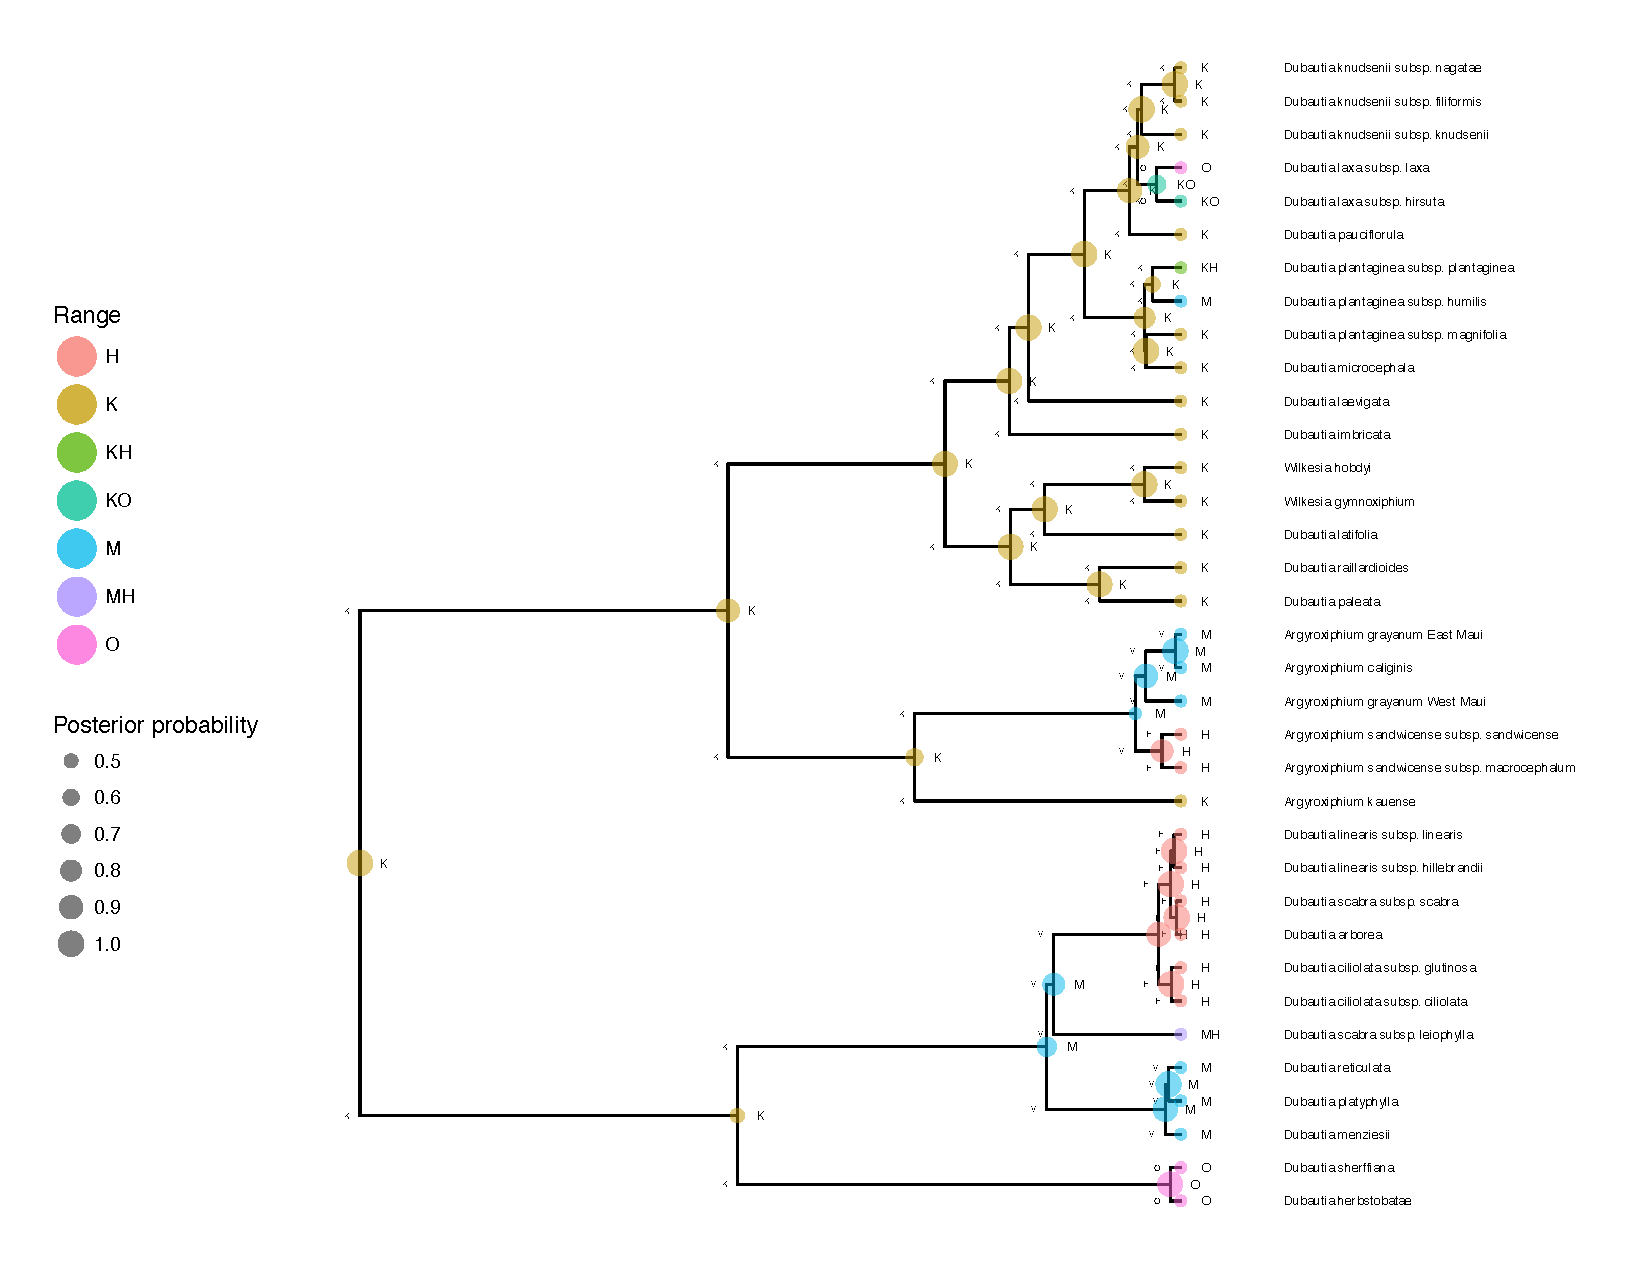
\includegraphics[width=0.75\textwidth]{figures/fig_epoch_RevGadgets_ase.pdf}
\caption{Tree with ancestral state estimates. Nodes are annotated with ancestral states before and after cladogenetic events. Most probable states are shown. Colors of markers indicate the range state. Sizes of markers indicate the posterior probability of that state. }
\label{fig:epoch_RevGadgets_ase}
\end{figure}

[ Look at posterior estimates for distance. ]

\newpage
